\documentclass[usenames,dvipsnames,xcolor=table]{beamer}
\usepackage[latin1]{inputenc}

\usecolortheme{beaver}
\usecolortheme{freiburg}

\usepackage{color, colortbl}
\usepackage{fancyvrb}
\usepackage{tikz}
\usepackage{float}
\usepackage{booktabs}
\usepackage{tikz}
\usetikzlibrary{calc, quotes, tikzmark, shapes,arrows,automata}
\beamertemplatenavigationsymbolsempty
\definecolor{dred}{rgb}{0.8, 0.0, 0.0}
\definecolor{uniblue}{HTML}{004a97}

%itemize label
%\setbeamercolor{item}{fg=uniblue}
%\textwidth = 290pt

\usepackage{xcolor}
\usepackage{listings}
\lstset{escapeinside={<@}{@>}}
\definecolor{gray}{rgb}{0.4,0.4,0.4}
\definecolor{darkblue}{rgb}{0.0,0.0,0.6}
\definecolor{cyan}{rgb}{0.0,0.6,0.3}
\definecolor{ALUblue}{rgb}{0,.42,.714}
\colorlet{ALUred}{red!70!black}
\definecolor{ALUgreen}{rgb}{.1,.5,0}
\definecolor{ALUblue}{rgb}{0,.42,.714}
\colorlet{ALUgray}{white!95!ALUblue}

\lstset{
  language=python,
  basicstyle=\scriptsize,
  columns=fullflexible,
  showstringspaces=false,
  commentstyle=\color{gray}\upshape
}

\usepackage{pgf}
\usepackage{pgfplotstable}
\usepackage{pgfplots}
\usepackage{mathtools}
\usepackage{xspace}
%------------------------------------------------------------------------------
%       (re)new commands / settings
%------------------------------------------------------------------------------
% ----------------- referencing ----------------

\newcommand{\multilineequation}[1]{\Bigl(\begin{matrix}#1\end{matrix}\Bigr)}


\usepackage{mathtools}
\usepackage[]{algorithmicx}
\usepackage[]{algorithm}
\usepackage{algpseudocode}
\usepackage{ stmaryrd }

\usetikzlibrary{shapes.misc, positioning}


\begin{document}
\title{UPGMA/WPGMA}
\subtitle{(Un)weighted \textcolor{ALUblue}{P}air \textcolor{ALUblue}{G}roup \textcolor{ALUblue}{M}ethod with \textcolor{ALUblue}{A}rithmetic Mean}
\author{Julian L\"offler}
\date{12.11.2018}
\frame{\titlepage}

\begin{frame}[fragile]
  \frametitle{Motivation for UPGMA / WPGMA}
  \begin{itemize}
    \item Consider a set of sequences:
    \begin{table}[]
      \begin{tabular}{ll}
        \textbf{A:} & TCAACTAC \\
        \textbf{B:} & ACTGCAAA \\
        \textbf{C:} & GGCTGTAA \\
        \textbf{D:} & AGTTGCAA \\
        \textbf{E:} & TTTGAACT
      \end{tabular}
    \end{table}
    \item The aim is \textcolor{ALUblue}{grouping} the most \textcolor{ALUblue}{similar sequences}, regardless of their evolutionary rate or phylogenetic affinities.
  \end{itemize}
\end{frame}

\begin{frame}[fragile]
  \frametitle{Motivation for UPGMA / WPGMA}
  \begin{itemize}
    \item \textcolor{ALUblue}{U}nweighted \textcolor{ALUblue}{P}air \textcolor{ALUblue}{G}roup \textcolor{ALUblue}{M}ethod with \textcolor{ALUblue}{A}rithmetic Mean
    \item \textcolor{ALUblue}{W}eighted \textcolor{ALUblue}{P}air \textcolor{ALUblue}{G}roup \textcolor{ALUblue}{M}ethod with \textcolor{ALUblue}{A}rithmetic Mean
    \item Used for the \textcolor{ALUblue}{creation of guide trees}.
  \end{itemize}
\end{frame}


\begin{frame}[fragile]
  \frametitle{UPGMA Algorithm}
  \begin{enumerate}
    \item Compute the \textcolor{ALUblue}{distance between each pair of sequences}.
    \item Treat \textcolor{ALUblue}{each sequence} as a \textcolor{ALUblue}{cluster $C$} by itself.
    \item \textcolor{ALUblue}{Merge the two closest clusters}. The distance between two clusters is the \textcolor{ALUred}{average distance between all their sequences}:
    $$d(C_i,C_j) = \frac{1}{|C_i| |C_j|} \sum_{r \in C_i, s\in C_j} d(r,s)$$
    \item Repeat 2. and 3. until only one cluster remains.vllt
  \end{enumerate}
\end{frame}

\begin{frame}
  \frametitle{Example}
  \begin{itemize}
    \item Let $\textcolor{ALUblue}{A},\textcolor{ALUblue}{B},\textcolor{ALUblue}{C},\textcolor{ALUblue}{D},\textcolor{ALUblue}{E}$ be sequences.
    \item Say we have calculated a distance matrix $D$:
  \end{itemize}
  \begin{table}[]
  \centering
  \begin{tabular}{c|c|c|c|c|c|}
  \cline{2-6}
                          & A & B & C & D & E \\ \hline
  \multicolumn{1}{|c|}{A} & 0 & 8 & 4 & 6 & 8 \\ \hline
  \multicolumn{1}{|c|}{B} & 8 & 0 & 8 & 8 & 4 \\ \hline
  \multicolumn{1}{|c|}{C} & 4 & 8 & 0 & 6 & 8 \\ \hline
  \multicolumn{1}{|c|}{D} & 6 & 8 & 6 & 0 & 8 \\ \hline
  \multicolumn{1}{|c|}{E} & 8 & 4 & 8 & 8 & 0 \\ \hline
  \end{tabular}
  \end{table}
\end{frame}

\begin{frame}[fragile]
  \frametitle{Example}
	\begin{itemize}
    \item Create guide tree for the \textcolor{ALUblue}{sequences}
	\end{itemize}
  \begin{columns}
  \begin{column}{0.5\textwidth}
    \begin{table}[]
    \centering
    \begin{tabular}{c|c|c|c|c|c|}
    \cline{2-6}
                            & A & B & C & D & E \\ \hline
    \multicolumn{1}{|c|}{A} & 0 & 8 & 4 & 6 & 8 \\ \hline
    \multicolumn{1}{|c|}{B} & 8 & 0 & 8 & 8 & 4 \\ \hline
    \multicolumn{1}{|c|}{C} & 4 & 8 & 0 & 6 & 8 \\ \hline
    \multicolumn{1}{|c|}{D} & 6 & 8 & 6 & 0 & 8 \\ \hline
    \multicolumn{1}{|c|}{E} & 8 & 4 & 8 & 8 & 0 \\ \hline
    \end{tabular}
    \end{table}
  \end{column}
  \begin{column}{0.5\textwidth}  %%<--- here
    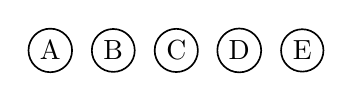
\begin{tikzpicture}[->,>=stealth',shorten >=1pt,auto,node distance=0.8cm,
        semithick,scale=1, every node/.style={scale=1}]
        \tikzstyle{every state}=[fill=white,draw=black,text=black,minimum size=5mm,inner sep=2pt]
        \node[state,align=center](A){A};
        \node[state,align=center](B)[right of=A]{B};
        \node[state,align=center](C)[right of=B]{C};
        \node[state,align=center](D)[right of=C]{D};
        \node[state,align=center](E)[right of=D]{E};
     \end{tikzpicture}
  \end{column}
  \end{columns}
\end{frame}

\begin{frame}[fragile]
  \frametitle{Example I}
	\begin{itemize}
		\item \textcolor{ALUblue}{\{A\}} and \textcolor{ALUblue}{\{C\}} are the closest clusters\\
		$\Rightarrow $ \textcolor{ALUgreen}{merge \{A\} and \{C\}  into \{A,C\}}.
		\item Each branch gets a total distance of $\frac{d(\{A\},\{C\})}{2} = \frac{4}{2}$.
	\end{itemize}
  \begin{columns}
  \begin{column}{0.5\textwidth}
    \begin{table}[]
    \centering
    \begin{tabular}{c|c|c|c|c|c|}
    \cline{2-6}
                                                                           & A & B & \cellcolor[HTML]{4B93C7}{\color[HTML]{EFEFEF} C} & D & E \\ \hline
    \multicolumn{1}{|c|}{\cellcolor[HTML]{4B93C7}{\color[HTML]{EFEFEF} A}} & 0 & 8 & \cellcolor[HTML]{F8A102}{\color[HTML]{000000} 4} & 6 & 8 \\ \hline
    \multicolumn{1}{|c|}{B}                                                & 8 & 0 & 8                                                & 8 & 4 \\ \hline
    \multicolumn{1}{|c|}{C}                                                & 4 & 8 & 0                                                & 6 & 8 \\ \hline
    \multicolumn{1}{|c|}{D}                                                & 6 & 8 & 6                                                & 0 & 8 \\ \hline
    \multicolumn{1}{|c|}{E}                                                & 8 & 4 & 8                                                & 8 & 0 \\ \hline
    \end{tabular}
    \end{table}
  \end{column}
  \begin{column}{0.5\textwidth}  %%<--- here
		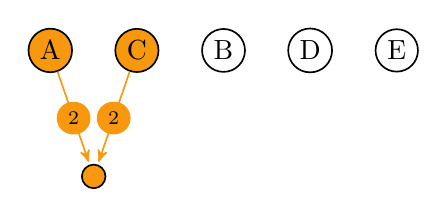
\begin{tikzpicture}[->,>=stealth',shorten >=1pt,auto,node distance=1.1cm,
        semithick,scale=1, every node/.style={scale=1}]
        \tikzstyle{every state}=[fill=white,draw=black,text=black,minimum size=3mm,inner sep=2pt]
        \node[state,align=center,fill=YellowOrange](A){A};
        \node[state,align=center, fill=YellowOrange](C)[right of=A]{C};
        \path (A) -- (C) coordinate[midway] (aux);
        \node[state,align=center, fill=YellowOrange, yshift=-0.5cm](AC)[below of=aux]{};
        \node[state,align=center](B)[right of=C]{B};
        \node[state,align=center](D)[right of=B]{D};
        \node[state,align=center](E)[right of=D]{E};
        \path (A) edge[draw=YellowOrange] node[anchor=center,align=center, draw=YellowOrange, fill=YellowOrange,rounded rectangle] {\scriptsize2} (AC);
        \path (C) edge[draw=YellowOrange] node[anchor=center,align=center, draw=YellowOrange, fill=YellowOrange,rounded rectangle] {\scriptsize2} (AC);
     \end{tikzpicture}
  \end{column}
  \end{columns}
\end{frame}

\begin{frame}[fragile]
  \frametitle{Example I}
	\begin{itemize}
		\item The distance between $\{A,C\}$ and the other clusters is the \textcolor{ALUred}{average distance between all their sequences}.
		\item Example: the new distance between $\{A,C\}$ and $\{B\}$ is:
    \scriptsize
		\begin{align*}
			d(\{A,C\}, \{B\}) &= \frac{1}{|\{A,C\}||\{B\}|}  (d(\{A\},\{B\}) + d(\{C\},\{B\}))\\
			                  &= \frac{1}{2} (8+8) = 8
		\end{align*}
	\end{itemize}
  \begin{columns}
		\tikzset{box/.style={inner xsep=0pt}}

		\begin{column}{0.5\textwidth}  %%<--- here
			\begin{table}[]
				\centering
				\begin{tabular}{c|c|c|c|c|c|}
					\cline{2-6}
					& A & B & \cellcolor[HTML]{4B93C7}{\color[HTML]{EFEFEF} C} & D & E \\ \hline
					\multicolumn{1}{|c|}{\cellcolor[HTML]{4B93C7}{\color[HTML]{EFEFEF} A}} & 0 & 8 & \cellcolor[HTML]{F8A102}{\color[HTML]{000000} 4} & 6 & 8 \\ \hline
					\multicolumn{1}{|c|}{B}                                                & 8 & 0 & 8                                                & 8 & 4 \\ \hline
					\multicolumn{1}{|c|}{C}                                                & 4 & 8 & 0                                                & 6 & 8\tikzmark{a}\\ \hline
					\multicolumn{1}{|c|}{D}                                                & 6 & 8 & 6                                                & 0 & 8 \\ \hline
					\multicolumn{1}{|c|}{E}                                                & 8 & 4 & 8                                                & 8 & 0 \\ \hline
				\end{tabular}
			\end{table}
		\end{column}
  \begin{column}{0.5\textwidth}
    \begin{table}[]
    \centering
    \begin{tabular}{c|c|c|c|c|}
    \cline{2-5}
                                                      & \cellcolor[HTML]{F8A102}A,C & B & D & E \\ \hline
    \multicolumn{1}{|c|}{\cellcolor[HTML]{F8A102}A,C} & 0                           & 8 & 6 & 8 \\  \hline
    \multicolumn{1}{|c|}{\tikzmark{b}B}                           & 8                           & 0 & 8 & 4 \\ \hline
    \multicolumn{1}{|c|}{D}                           & 6                           & 8 & 0 & 8 \\ \hline
    \multicolumn{1}{|c|}{E}                           & 8                           & 4 & 8 & 0 \\ \hline
    \end{tabular}
    \end{table}
  \end{column}
  \end{columns}
	
\begin{tikzpicture}[overlay,remember picture,->]
    \draw[very thick]         ($({pic cs:a})+(4.0ex,1ex)$)
        to   ($({pic cs:b})+(-4.8ex,-0.4ex)$);
    \end{tikzpicture}
\end{frame}

\begin{frame}[fragile]
  \frametitle{Example II}
	\begin{itemize}
		\item \textcolor{ALUblue}{\{B\}} and \textcolor{ALUblue}{\{E\}} are the closest clusters\\
		$\Rightarrow $ \textcolor{ALUgreen}{merge \{B\} and \{E\}  into \{B,E\}}.
		\item Assign $\frac{d(\{B\},\{E\})}{2} = \frac{4}{2} = 2$ to each branch.
	\end{itemize}
  \begin{columns}
  \begin{column}{0.5\textwidth}
    \begin{table}[]
    \centering
    \begin{tabular}{c|c|c|c|c|}
    \cline{2-5}
                                                      & \cellcolor[HTML]{FFFFFF}A,C & B & D & \cellcolor[HTML]{4B93C7}E \\ \hline
    \multicolumn{1}{|c|}{\cellcolor[HTML]{FFFFFF}A,C} & 0                           & 8 & 6 & 8                         \\ \hline
    \multicolumn{1}{|c|}{\cellcolor[HTML]{4B93C7}B}   & 8                           & 0 & 8 & \cellcolor[HTML]{F8A102}4 \\ \hline
    \multicolumn{1}{|c|}{D}                           & 6                           & 8 & 0 & 8                         \\ \hline
    \multicolumn{1}{|c|}{E}                           & 8                           & 4 & 8 & 0                         \\ \hline
    \end{tabular}
    \end{table}
  \end{column}
  \begin{column}{0.5\textwidth}  %%<--- here
		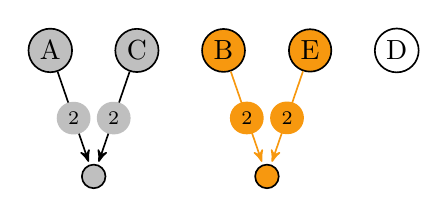
\begin{tikzpicture}[->,>=stealth',shorten >=1pt,auto,node distance=1.1cm,
        semithick,scale=1, every node/.style={scale=1}]
        \tikzstyle{every state}=[fill=white,draw=black,text=black,minimum size=3mm,inner sep=2pt]
        \node[state,align=center, fill=lightgray](A){A};
        \node[state,align=center,fill=lightgray](C)[right of=A]{C};
        \path (A) -- (C) coordinate[midway] (aux);
        \node[state,align=center, fill=lightgray, yshift=-0.5cm](AC)[below of=aux]{};
        \node[state,align=center, fill=YellowOrange](B)[right of=C]{B};
        \node[state,align=center, fill=YellowOrange](E)[right of=B]{E};
        \path (B) -- (E) coordinate[midway] (aux2);
        \node[state,align=center, fill=YellowOrange, yshift=-0.5cm](BE)[below of=aux2]{};
        \node[state,align=center](D)[right of=E]{D};
        \path (A) edge[draw=black] node[anchor=center,align=center, draw=lightgray, fill=lightgray,rounded rectangle] {\scriptsize2} (AC);
        \path (C) edge[draw=black] node[anchor=center,align=center, draw=lightgray, fill=lightgray,rounded rectangle] {\scriptsize2} (AC);
        \path (B) edge[draw=YellowOrange] node[anchor=center,align=center, draw=YellowOrange, fill=YellowOrange,rounded rectangle] {\scriptsize2} (BE);
        \path (E) edge[draw=YellowOrange] node[anchor=center,align=center, draw=YellowOrange, fill=YellowOrange,rounded rectangle] {\scriptsize2} (BE);
     \end{tikzpicture}
  \end{column}
  \end{columns}
\end{frame}

\begin{frame}[fragile]
  \frametitle{Example II}
	\begin{itemize}
		\item The distance between $\{B,E\}$ and the other clusters is the \textcolor{ALUred}{average distance between all their sequences}.

	\end{itemize}
  \begin{columns}
		\tikzset{box/.style={inner xsep=0pt}}
		\begin{column}{0.5\textwidth}  %%<--- here
			\begin{table}[]
				\centering
				\begin{tabular}{c|c|c|c|c|}
					\cline{2-5}
					& \cellcolor[HTML]{FFFFFF}A,C & B & D & \cellcolor[HTML]{4B93C7}E \\ \hline
					\multicolumn{1}{|c|}{\cellcolor[HTML]{FFFFFF}A,C} & 0                           & 8 & 6 & 8                         \\ \hline
					\multicolumn{1}{|c|}{\cellcolor[HTML]{4B93C7}B}   & 8                           & 0 & 8 & \cellcolor[HTML]{F8A102}4\tikzmark{c} \\ \hline
					\multicolumn{1}{|c|}{D}                           & 6                           & 8 & 0 & 8                         \\ \hline
					\multicolumn{1}{|c|}{E}                           & 8                           & 4 & 8 & 0                         \\ \hline
				\end{tabular}
			\end{table}
		\end{column}
  \begin{column}{0.5\textwidth}
    \begin{table}[]
  \centering
  \begin{tabular}{c|c|c|c|}
  \cline{2-4}
                                                    & \cellcolor[HTML]{FFFFFF}A,C & \cellcolor[HTML]{F8A102}B,E & D \\ \hline
  \multicolumn{1}{|c|}{\tikzmark{d}\cellcolor[HTML]{FFFFFF}A,C} & 0                           & 8                           & 6 \\ \hline
  \multicolumn{1}{|c|}{\cellcolor[HTML]{F8A102}B,E} & 8                           & 0                           & 8 \\ \hline
  \multicolumn{1}{|c|}{D}                           & 6                           & 8                           & 0 \\ \hline
  \end{tabular}
  \end{table}
  \end{column}
  \end{columns}
	
\begin{tikzpicture}[overlay,remember picture,->]
    \draw[very thick]         ($({pic cs:c})+(4.0ex,1ex)$)
        to   ($({pic cs:d})+(-4.8ex,-0.4ex)$);
    \end{tikzpicture}
\end{frame}

\begin{frame}[fragile]
  \frametitle{Example III}
	\begin{itemize}
		\item \textcolor{ALUblue}{\{A,C\}} and \textcolor{ALUblue}{\{D\}} are the closest clusters\\
		$\Rightarrow $ \textcolor{ALUgreen}{merge \{A,C\} and \{D\}  into \{A,C,D\}}.
		\item Assign $\frac{d(\{A,C\}, \{D\})}{2} = \frac{6}{2} = 3$ total length to each branch.
		\item Observe, that the 1 is obtained calculating $3-\textcolor{ALUred}{2} = 1$.
	\end{itemize}
  \begin{columns}
  \begin{column}{0.5\textwidth}
    \begin{table}[]
  \centering
  \begin{tabular}{c|c|c|c|}
  \cline{2-4}
                                                    & \cellcolor[HTML]{FFFFFF}A,C & \cellcolor[HTML]{FFFFFF}B,E & \cellcolor[HTML]{4B93C7}D \\ \hline
  \multicolumn{1}{|c|}{\cellcolor[HTML]{4B93C7}A,C} & 0                           & 8                           & \cellcolor[HTML]{F8A102}6 \\ \hline
  \multicolumn{1}{|c|}{\cellcolor[HTML]{FFFFFF}B,E} & 8                           & 0                           & 8                         \\ \hline
  \multicolumn{1}{|c|}{D}                           & 6                           & 8                           & 0                         \\ \hline
  \end{tabular}
  \end{table}
  \end{column}
  \begin{column}{0.5\textwidth}  %%<--- here
		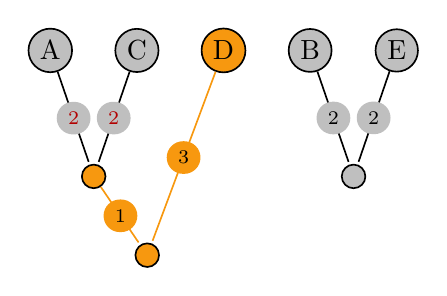
\begin{tikzpicture}[-,>=stealth',shorten >=1pt,auto,node distance=1.1cm,
        semithick,scale=1, every node/.style={scale=1}]
        \tikzstyle{every state}=[fill=white,draw=black,text=black,minimum size=3mm,inner sep=2pt]
        \node[state,align=center, fill=lightgray](A){A};
        \node[state,align=center,fill=lightgray](C)[right of=A]{C};
        \node[state,align=center, fill=YellowOrange](D)[right of=C]{D};
        \path (A) -- (C) coordinate[midway] (aux);
        \path (aux) -- (D) coordinate[midway] (aux3);
        \node[state,align=center, fill=YellowOrange, yshift=-0.5cm](AC)[below of=aux]{};
        \node[state,align=center, fill=YellowOrange, yshift=-1.5cm](ACD)[below of=aux3]{};
        \node[state,align=center, fill=lightgray](B)[right of=D]{B};
        \node[state,align=center, fill=lightgray](E)[right of=B]{E};
        \path (B) -- (E) coordinate[midway] (aux2);
        \node[state,align=center, fill=lightgray, yshift=-0.5cm](BE)[below of=aux2]{};
        \path (A) edge[draw=black] node[anchor=center,align=center, draw=lightgray, fill=lightgray,rounded rectangle] {\scriptsize\textcolor{ALUred}{2}} (AC);
        \path (C) edge[draw=black] node[anchor=center,align=center, draw=lightgray, fill=lightgray,rounded rectangle] {\scriptsize\textcolor{ALUred}{2}} (AC);

        \path (AC) edge[draw=YellowOrange] node[anchor=center,align=center, draw=YellowOrange, fill=YellowOrange,rounded rectangle] {\scriptsize1} (ACD);
        \path (D) edge[draw=YellowOrange] node[anchor=center,align=center, draw=YellowOrange, fill=YellowOrange,rounded rectangle] {\scriptsize3} (ACD);

        \path (B) edge[draw=black] node[anchor=center,align=center, draw=lightgray, fill=lightgray,rounded rectangle] {\scriptsize2} (BE);
        \path (E) edge[draw=black] node[anchor=center,align=center, draw=lightgray, fill=lightgray,rounded rectangle] {\scriptsize2} (BE);
     \end{tikzpicture}
  \end{column}
  \end{columns}
\end{frame}

\begin{frame}[fragile]
  \frametitle{Example III}
	\begin{itemize}
		\item The distance between \textcolor{ALUblue}{$\{A,C,D\}$} and \textcolor{ALUblue}{$\{B,E\}$} is the \textcolor{ALUred}{average distance between all their sequences}.
	\end{itemize}
  \begin{columns}
		\tikzset{box/.style={inner xsep=0pt}}
		\begin{column}{0.5\textwidth}  %%<--- here
			\begin{table}[]
				\centering
				\begin{tabular}{c|c|c|c|}
					\cline{2-4}
					& \cellcolor[HTML]{FFFFFF}A,C & \cellcolor[HTML]{FFFFFF}B,E & \cellcolor[HTML]{4B93C7}D \\ \hline
					\multicolumn{1}{|c|}{\cellcolor[HTML]{4B93C7}A,C} & 0                           & 8                           & \cellcolor[HTML]{F8A102}6 \\ \hline
					\multicolumn{1}{|c|}{\cellcolor[HTML]{FFFFFF}B,E} & 8                           & 0                           & 8\tikzmark{e}                         \\ \hline
					\multicolumn{1}{|c|}{D}                           & 6                           & 8                           & 0                         \\ \hline
				\end{tabular}
			\end{table}
		\end{column}
  \begin{column}{0.5\textwidth}
    \begin{table}[]
  \centering
  \begin{tabular}{c|c|c|}
  \cline{2-3}
                                                      & \cellcolor[HTML]{F8A102}A,C,D & B,E \\ \hline
  \multicolumn{1}{|c|}{\tikzmark{f}\cellcolor[HTML]{F8A102}A,C,D} & 0                             & 8   \\ \hline
  \multicolumn{1}{|c|}{\cellcolor[HTML]{FFFFFF}B,E}   & 8                             & 0   \\ \hline
  \end{tabular}
  \end{table}
  \end{column}
  \end{columns}
	
\begin{tikzpicture}[overlay,remember picture,->]
    \draw[very thick]         ($({pic cs:e})+(4.0ex,1ex)$)
        to   ($({pic cs:f})+(-4.8ex,-0.4ex)$);
    \end{tikzpicture}
\end{frame}

\begin{frame}[fragile]
  \frametitle{Example IV}
	\begin{itemize}
		\item \textcolor{ALUblue}{\{A,C, D\}} and \textcolor{ALUblue}{\{B,E\}} are remaining.\\
		$\Rightarrow $ \textcolor{ALUgreen}{merge \{A,C,D\} and \{B,E\}  into \{A,C,D, B, E\}}.
	\end{itemize}
  \begin{columns}
  \begin{column}{0.5\textwidth}
    \begin{table}[]
    \centering
    \begin{tabular}{c|c|c|}
    \cline{2-3}
                                                        & A,C,D & \cellcolor[HTML]{4B93C7}B,E \\ \hline
    \multicolumn{1}{|c|}{\cellcolor[HTML]{4B93C7}A,C,D} & 0     & \cellcolor[HTML]{F8A102}8   \\ \hline
    \multicolumn{1}{|c|}{\cellcolor[HTML]{FFFFFF}B,E}   & 8     & 0                           \\ \hline
    \end{tabular}
    \end{table}
  \end{column}
  \begin{column}{0.5\textwidth}  %%<--- here
    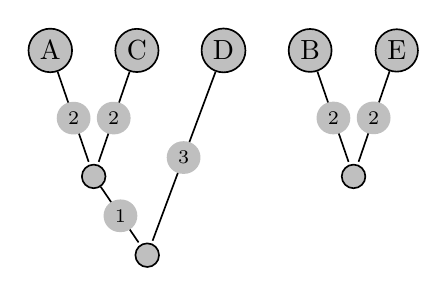
\begin{tikzpicture}[-,>=stealth',shorten >=1pt,auto,node distance=1.1cm,
        semithick,scale=1, every node/.style={scale=1}]
        \tikzstyle{every state}=[fill=white,draw=black,text=black,minimum size=3mm,inner sep=2pt]
        \node[state,align=center, fill=lightgray](A){A};
        \node[state,align=center,fill=lightgray](C)[right of=A]{C};
        \node[state,align=center, fill=lightgray](D)[right of=C]{D};
        \path (A) -- (C) coordinate[midway] (aux);
        \path (aux) -- (D) coordinate[midway] (aux3);
        \node[state,align=center, fill=lightgray, yshift=-0.5cm](AC)[below of=aux]{};
        \node[state,align=center, fill=lightgray, yshift=-1.5cm](ACD)[below of=aux3]{};
        \node[state,align=center, fill=lightgray](B)[right of=D]{B};
        \node[state,align=center, fill=lightgray](E)[right of=B]{E};
        \path (B) -- (E) coordinate[midway] (aux2);
        \node[state,align=center, fill=lightgray, yshift=-0.5cm](BE)[below of=aux2]{};
        \path (A) edge[draw=black] node[anchor=center,align=center, draw=lightgray, fill=lightgray,rounded rectangle] {\scriptsize2} (AC);
        \path (C) edge[draw=black] node[anchor=center,align=center, draw=lightgray, fill=lightgray,rounded rectangle] {\scriptsize2} (AC);

        \path (AC) edge[draw=black] node[anchor=center,align=center, draw=lightgray, fill=lightgray,rounded rectangle] {\scriptsize1} (ACD);
        \path (D) edge[draw=black] node[anchor=center,align=center, draw=lightgray, fill=lightgray,rounded rectangle] {\scriptsize3} (ACD);

        \path (B) edge[draw=black] node[anchor=center,align=center, draw=lightgray, fill=lightgray,rounded rectangle] {\scriptsize2} (BE);
        \path (E) edge[draw=black] node[anchor=center,align=center, draw=lightgray, fill=lightgray,rounded rectangle] {\scriptsize2} (BE);
     \end{tikzpicture}
  \end{column}
  \end{columns}
\end{frame}

\begin{frame}[fragile]
  \frametitle{Example IV}
	\begin{itemize}
		\item Assign $\frac{d(\{A,C, D\}, \{B,E\})}{2} = \frac{8}{2} = 4$ total length to each branch.
		\item Observe, that the 1 is obtained calculating $4-\textcolor{ALUred}{3} = 1$.
		\item Observe, that the 2 is obtained calculating $4-\textcolor{ALUgreen}{2} = 2$.
	\end{itemize}
  \begin{columns}
  \begin{column}{0.5\textwidth}
    \begin{table}[]
    \centering
    \begin{tabular}{c|c|}
    \cline{2-2}
                                                            & \cellcolor[HTML]{F8A102}A,C,D,B,E \\ \hline
    \multicolumn{1}{|c|}{\cellcolor[HTML]{F8A102}A,C,D,B,E} & 0                                 \\ \hline
    \end{tabular}
    \end{table}
  \end{column}
  \begin{column}{0.5\textwidth}  %%<--- here
    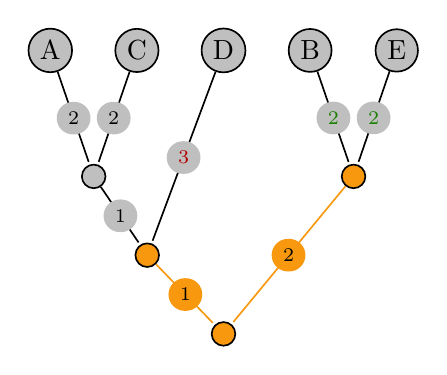
\begin{tikzpicture}[-,>=stealth',shorten >=1pt,auto,node distance=1.1cm,
        semithick,scale=1, every node/.style={scale=1}]
        \tikzstyle{every state}=[fill=white,draw=black,text=black,minimum size=3mm,inner sep=2pt]
        \node[state,align=center, fill=lightgray](A){A};
        \node[state,align=center,fill=lightgray](C)[right of=A]{C};
        \node[state,align=center, fill=lightgray](D)[right of=C]{D};
        \path (A) -- (C) coordinate[midway] (aux);
        \path (aux) -- (D) coordinate[midway] (aux3);
        \node[state,align=center, fill=lightgray, yshift=-0.5cm](AC)[below of=aux]{};
        \node[state,align=center, fill=YellowOrange, yshift=-1.5cm](ACD)[below of=aux3]{};
        \node[state,align=center, fill=lightgray](B)[right of=D]{B};
        \node[state,align=center, fill=lightgray](E)[right of=B]{E};
        \path (B) -- (E) coordinate[midway] (aux2);
        \node[state,align=center, fill=YellowOrange, yshift=-0.5cm](BE)[below of=aux2]{};
        \node[state,align=center, fill=YellowOrange, yshift=-2.5cm](ACDBE)[below of=D]{};

        \path (A) edge[draw=black] node[anchor=center,align=center, draw=lightgray, fill=lightgray,rounded rectangle] {\scriptsize2} (AC);
        \path (C) edge[draw=black] node[anchor=center,align=center, draw=lightgray, fill=lightgray,rounded rectangle] {\scriptsize2} (AC);

        \path (AC) edge[draw=black] node[anchor=center,align=center, draw=lightgray, fill=lightgray,rounded rectangle] {\scriptsize1} (ACD);
        \path (D) edge[draw=black] node[anchor=center,align=center, draw=lightgray, fill=lightgray,rounded rectangle] {\scriptsize\textcolor{ALUred}{3}} (ACD);

        \path (B) edge[draw=black] node[anchor=center,align=center, draw=lightgray, fill=lightgray,rounded rectangle] {\scriptsize\textcolor{ALUgreen}{2}} (BE);
        \path (E) edge[draw=black] node[anchor=center,align=center, draw=lightgray, fill=lightgray,rounded rectangle] {\scriptsize\textcolor{ALUgreen}{2}} (BE);
        \path (ACD) edge[draw=YellowOrange] node[anchor=center,align=center, draw=YellowOrange, fill=YellowOrange,rounded rectangle] {\scriptsize1} (ACDBE);
        \path (BE) edge[draw=YellowOrange] node[anchor=center,align=center, draw=YellowOrange, fill=YellowOrange,rounded rectangle] {\scriptsize2} (ACDBE);
     \end{tikzpicture}
  \end{column}
  \end{columns}
\end{frame}

\begin{frame}[fragile]
  \frametitle{Example V}
	\begin{itemize}
		\item Our beautiful tree:
	\end{itemize}
    \begin{center}
      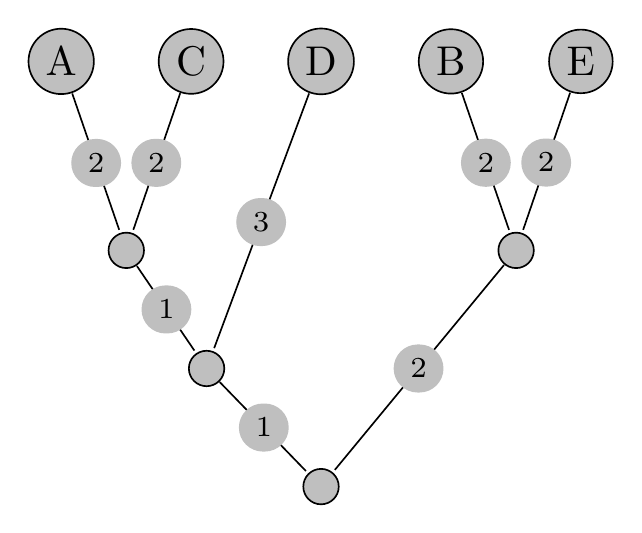
\begin{tikzpicture}[-,>=stealth',shorten >=1pt,auto,node distance=1.1cm,
        semithick,scale=1, every node/.style={scale=1.5}]
        \tikzstyle{every state}=[fill=white,draw=black,text=black,minimum size=3mm,inner sep=2pt]
        \node[state,align=center, fill=lightgray](A){A};
        \node[state,align=center,fill=lightgray](C)[right of=A]{C};
        \node[state,align=center, fill=lightgray](D)[right of=C]{D};
        \path (A) -- (C) coordinate[midway] (aux);
        \path (aux) -- (D) coordinate[midway] (aux3);
        \node[state,align=center, fill=lightgray, yshift=-0.5cm](AC)[below of=aux]{};
        \node[state,align=center, fill=lightgray, yshift=-1.5cm](ACD)[below of=aux3]{};
        \node[state,align=center, fill=lightgray](B)[right of=D]{B};
        \node[state,align=center, fill=lightgray](E)[right of=B]{E};
        \path (B) -- (E) coordinate[midway] (aux2);
        \node[state,align=center, fill=lightgray, yshift=-0.5cm](BE)[below of=aux2]{};
        \node[state,align=center, fill=lightgray, yshift=-2.5cm](ACDBE)[below of=D]{};

        \path (A) edge[draw=black] node[anchor=center,align=center, draw=lightgray, fill=lightgray,rounded rectangle] {\scriptsize2} (AC);
        \path (C) edge[draw=black] node[anchor=center,align=center, draw=lightgray, fill=lightgray,rounded rectangle] {\scriptsize2} (AC);

        \path (AC) edge[draw=black] node[anchor=center,align=center, draw=lightgray, fill=lightgray,rounded rectangle] {\scriptsize1} (ACD);
        \path (D) edge[draw=black] node[anchor=center,align=center, draw=lightgray, fill=lightgray,rounded rectangle] {\scriptsize3} (ACD);

        \path (B) edge[draw=black] node[anchor=center,align=center, draw=lightgray, fill=lightgray,rounded rectangle] {\scriptsize2} (BE);
        \path (E) edge[draw=black] node[anchor=center,align=center, draw=lightgray, fill=lightgray,rounded rectangle] {\scriptsize2} (BE);
        \path (ACD) edge[draw=black] node[anchor=center,align=center, draw=lightgray, fill=lightgray,rounded rectangle] {\scriptsize1} (ACDBE);
        \path (BE) edge[draw=black] node[anchor=center,align=center, draw=lightgray, fill=lightgray,rounded rectangle] {\scriptsize2} (ACDBE);
      \end{tikzpicture}
    \end{center}
\end{frame}


  	\frame{
  		\frametitle{WPGMA}
  		\begin{itemize}
  		\item In \textcolor{ALUblue}{WPGMA} the \textcolor{ALUblue}{distance between clusters} is calculated as a \textcolor{ALUblue}{simple average}:
			$$d(C_i \cup C_j, C_k) = \frac{d(C_i,C_k) + d(C_j,C_k)}{2}$$
			\item Computationally easier than  \textcolor{ALUblue}{UPGMA}.
		 \item \textcolor{ALUred}{Unequal numbers of taxa} in the clusters cause problems\\
		 $\Rightarrow$ the distances in the original matrix \textcolor{ALUred}{do not contribute equally} to the intermediate calculations.
		 \item The branches do not preserve the original distances.
		 \item Final result is therefore said to be \textcolor{ALUblue}{weighted}.
  		\end{itemize}
  	}


  	\frame{
  		\frametitle{Final notes}
  		\begin{itemize}
  		\item Clustering works only if the data are \textcolor{ALUblue}{ultrametric}.
			\item Ultrametric distances are defined by the satisfaction of the \textcolor{ALUblue}{three-point condition}:
			\begin{itemize}
				\item For any three taxa it holds:
				$$d(A, C) \leq max(d(A,B), d(B,C))$$
			\end{itemize}
			\item So we assume that all taxa evolve with the same constant rate
				\item $O(n^3)$ for the trivial approach.
				\item $O(n^2 log(n))$, when using a heap for each cluster
				\item $O(k 3^k n^2) / O(n^2)$ implementations for special cases. (by Fionn Murtagh,  by Day and Edelsbrunner)
  		\end{itemize}
  	}

			\frame{
				\frametitle{References}
				The content of this set of slides, is based on:
				\begin{itemize}

				\item Construction of a distance tree using clustering with the Unweighted Pair Group Method with Arithmatic Mean (UPGMA):
				\url{https://www.icp.ucl.ac.be/~opperd/private/upgma.html}
				\item UPGMA Wikipedia article:
				\url{https://en.wikipedia.org/wiki/UPGMA}
				\item WPGMA:
				\url{http://www.wikiwand.com/en/WPGMA}
				\end{itemize}
			}

\end{document}
